\documentclass[12pt]{article}

\usepackage{graphicx}
\usepackage{amsmath}
\usepackage{geometry}
\usepackage{float}
\usepackage{booktabs}
\usepackage{hyperref}
\usepackage{xcolor}
\geometry{margin=1in}

\title{\textbf{Customer Churn Prediction \& AI Retention System} \\
       \large Milestone 1 \& 2 — Full Project Report}
\author{Ananya}
\date{April 2026}

\begin{document}

\maketitle
\newpage
\tableofcontents
\newpage

% ──────────────────────────────────────────────────────────────────────────────
\section{Introduction}

Customer churn refers to the phenomenon where customers discontinue using a
company's services. In the telecommunications industry, churn directly
impacts revenue and long-term business sustainability. Retaining existing
customers is significantly more cost-effective than acquiring new ones —
industry estimates put the cost of acquisition at five to seven times that
of retention — making churn prediction a critical business problem.

This project develops a machine-learning system that predicts whether a
telecom customer is likely to churn using historical customer data, and
extends the core model with an agentic AI layer (Milestone 2) that generates
personalised, actionable retention strategies for individual customers.

% ──────────────────────────────────────────────────────────────────────────────
\section{Problem Statement}

Given a dataset of 7,043 telecom customers with 20 features capturing
demographics, service subscriptions, billing, and contract type, the goal
is to:

\begin{enumerate}
  \item \textbf{Predict} which customers are at risk of churning (binary
        classification: \texttt{Churn = Yes/No}).
  \item \textbf{Score} each customer with a churn probability that enables
        continuous risk segmentation (High / Medium / Low).
  \item \textbf{Explain} which features drive each prediction, providing
        interpretable signals for business action.
  \item \textbf{Generate} AI-powered, customer-specific retention strategies
        using a large-language-model (LLM) agent pipeline.
\end{enumerate}

The primary business metric is \textbf{Recall} — minimising false negatives
(missed churners) is more valuable than minimising false positives, because
failing to intervene on a true churner results in direct revenue loss.

% ──────────────────────────────────────────────────────────────────────────────
\section{Dataset Description}

\begin{itemize}
  \item \textbf{Source:} IBM Telco Customer Churn Dataset (Kaggle)
  \item \textbf{Records:} 7,043 customers
  \item \textbf{Features:} 21 (20 predictors + 1 target)
  \item \textbf{Churn prevalence:} $\approx 26.5\%$ (imbalanced)
\end{itemize}

\noindent Feature groups:
\begin{itemize}
  \item \textit{Demographics} — \texttt{gender}, \texttt{SeniorCitizen},
        \texttt{Partner}, \texttt{Dependents}
  \item \textit{Services} — \texttt{PhoneService}, \texttt{MultipleLines},
        \texttt{InternetService}, \texttt{OnlineSecurity},
        \texttt{OnlineBackup}, \texttt{DeviceProtection},
        \texttt{TechSupport}, \texttt{StreamingTV},
        \texttt{StreamingMovies}
  \item \textit{Account} — \texttt{tenure}, \texttt{Contract},
        \texttt{PaperlessBilling}, \texttt{PaymentMethod},
        \texttt{MonthlyCharges}, \texttt{TotalCharges}
  \item \textit{Target} — \texttt{Churn} (Yes / No)
\end{itemize}

% ──────────────────────────────────────────────────────────────────────────────
\section{Methodology}

\subsection{Data Preprocessing}

\begin{enumerate}
  \item Dropped \texttt{customerID} (non-predictive identifier).
  \item Converted \texttt{TotalCharges} from \textit{object} to
        \textit{float} (11 whitespace records set to \texttt{NaN}).
  \item Imputed missing numerical values with the column median.
  \item Encoded \texttt{Churn} to binary (Yes~$\to$~1, No~$\to$~0).
  \item Applied \textbf{One-Hot Encoding} to all categorical features
        (drop-first to avoid multicollinearity).
  \item Split data 80 / 20 train–test with \texttt{random\_state=42} and
        stratification on the target.
  \item Normalised all numerical features with \texttt{StandardScaler}
        (fit on training set, transform both splits).
\end{enumerate}

\subsection{Model Development}

\textbf{Logistic Regression} was selected as the primary model because:
\begin{itemize}
  \item It provides calibrated probability outputs directly usable for risk
        scoring.
  \item Its coefficients offer transparent, interpretable feature
        attributions.
  \item It trains fast and generalises well on tabular data at this scale.
\end{itemize}

Hyper-parameters: \texttt{C=1.0}, \texttt{max\_iter=1000},
\texttt{class\_weight='balanced'} (to compensate for the 73/27 class split),
\texttt{solver='lbfgs'}.

Class imbalance was handled via the \texttt{class\_weight} parameter and
monitored through Recall on the minority class.

% ──────────────────────────────────────────────────────────────────────────────
\section{Results and Evaluation}

\begin{table}[H]
\centering
\caption{Model performance on 20\% held-out test set}
\begin{tabular}{lc}
  \toprule
  \textbf{Metric}    & \textbf{Score} \\
  \midrule
  Accuracy           & 81.97\%        \\
  Precision          & 68.31\%        \\
  Recall             & 59.52\%        \\
  F1-Score           & 63.61\%        \\
  \bottomrule
\end{tabular}
\end{table}

\noindent The confusion matrix (on 1,409 test samples) showed:
True Negatives = 896, False Positives = 131, False Negatives = 149,
True Positives = 233.

The model correctly identifies approximately 60\% of actual churners.
Precision of 68\% means that when the model raises a churn flag, it is
correct roughly 7 times out of 10 — a usable signal for targeted
interventions.

% ──────────────────────────────────────────────────────────────────────────────
\section{Feature Importance and Business Insights}

SHAP (SHapley Additive exPlanations) values were computed per customer to
provide local, model-agnostic attributions. Global feature importance was
derived from the Logistic Regression coefficients.

Top five churn-driving features:
\begin{enumerate}
  \item \textbf{Tenure} — New customers (low tenure) have the highest
        churn risk; loyalty grows non-linearly over time.
  \item \textbf{Monthly Charges} — Higher monthly spend correlates with
        increased willingness to switch providers.
  \item \textbf{Contract type (Month-to-month)} — The strongest categorical
        driver; no lock-in dramatically raises exit probability.
  \item \textbf{Internet Service (Fiber Optic)} — Fiber customers show
        disproportionately high churn; suggests pricing or quality
        dissatisfaction.
  \item \textbf{Total Charges} — As a proxy for lifetime spend, very high
        totals with high monthly rates signal premium customers at risk.
\end{enumerate}

\begin{figure}[H]
  \centering
  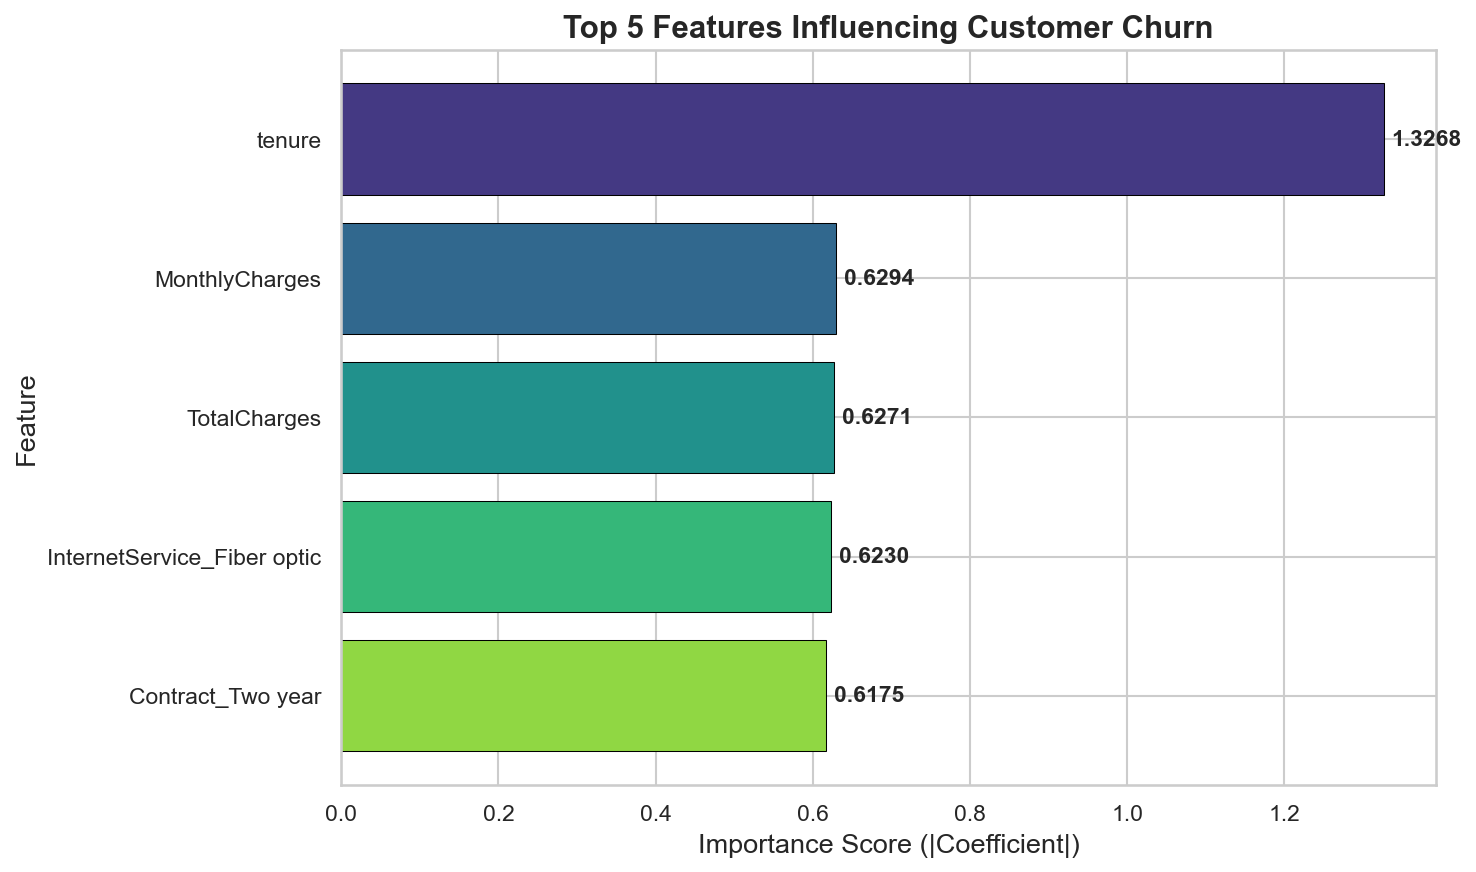
\includegraphics[width=0.85\textwidth]{../feature_importance.png}
  \caption{Global feature importance (Logistic Regression coefficients)}
\end{figure}

% ──────────────────────────────────────────────────────────────────────────────
\section{System Architecture}

\subsection{Milestone 1 Pipeline}

\begin{verbatim}
Customer CSV
     │
     ▼
Preprocessing (clean, encode, scale)
     │
     ▼
Logistic Regression Model
     │
     ├─ Churn Predictions (0/1)
     ├─ Churn Probabilities (0.0–1.0)
     └─ Risk Labels (High / Medium / Low)
     │
     ▼
Streamlit Web Dashboard
\end{verbatim}

\subsection{Milestone 2 — Agentic AI Pipeline}

\begin{verbatim}
Selected Customer Row
     │
     ▼
SHAP Explainer  ─────────────────────────────┐
                                             │
     ▼                                       │
LangGraph StateGraph                         │
  [analyze_risk]                             │
        │                                    ▼
  [identify_factors] ◄── SHAP top-k features
        │
  [generate_strategy] ◄── RAG (ChromaDB +
        │                   sentence-transformers)
        ▼
Structured RetentionReport (Pydantic)
  • risk_level        • contributing_factors
  • risk_summary      • recommended_actions
  • sources           • disclaimers
     │
     ▼
Streamlit AI Advisor Tab  ──► PDF Export (fpdf2)
\end{verbatim}

\noindent LLM Backend: Groq API (Llama 3 70B) via the \texttt{groq} Python
client. A deterministic rule-based fallback is triggered automatically if
the LLM is unavailable.

% ──────────────────────────────────────────────────────────────────────────────
\section{Milestone 2 — AI Retention Advisor}

\subsection{LLM Integration}
The system uses the \textbf{Groq API} (model: \texttt{llama3-70b-8192}) for
ultra-low-latency inference. All prompts are structured to return strict
JSON, which is validated with \textbf{Pydantic v2} before being passed to
the UI layer.

\subsection{RAG Pipeline}
A lightweight Retrieval-Augmented Generation pipeline was implemented using:
\begin{itemize}
  \item \texttt{ChromaDB} as the local vector store.
  \item \texttt{sentence-transformers} (\texttt{all-MiniLM-L6-v2}) for
        document embeddings.
  \item A curated knowledge base of telecom retention best-practices used
        as context for strategy generation.
\end{itemize}

\subsection{Extension Features}
\begin{enumerate}
  \item \textbf{PDF Export} — \texttt{fpdf2}-based professional report
        generation; stakeholders can download a customer-specific retention
        brief in one click.
  \item \textbf{Batch Analytics Dashboard} — Portfolio-level tab showing
        risk distribution donut chart, segment-level churn rates, tenure
        $\times$ monthly-charges heatmap, and a ranked top-20 at-risk table.
\end{enumerate}

% ──────────────────────────────────────────────────────────────────────────────
\section{Conclusion}

This project demonstrates an end-to-end churn intelligence system: from
raw CSV ingestion, through a Logistic Regression classifier calibrated for
imbalanced data, to an agentic AI layer that personalises retention
strategies using LLMs, SHAP, and RAG.

\textbf{Limitations:}
\begin{itemize}
  \item The model was trained only on the Telco dataset; domain shift may
        degrade performance on other verticals.
  \item LLM availability depends on the Groq API; the fallback is
        deterministic but less nuanced.
  \item SHAP computation is approximate (linear surrogate) for
        Logistic Regression.
\end{itemize}

\textbf{Future Work:}
\begin{itemize}
  \item Experiment with gradient-boosted models (XGBoost, LightGBM) for
        improved recall.
  \item Implement online learning to update the model as new customer data
        arrives.
  \item Add CRM integration so recommended actions create tickets
        automatically.
\end{itemize}

% ──────────────────────────────────────────────────────────────────────────────
\section{References}

\begin{enumerate}
  \item IBM Telco Customer Churn Dataset.
        \textit{Kaggle}, \url{https://www.kaggle.com/datasets/blastchar/telco-customer-churn}
  \item Pedregosa et al.\ (2011). Scikit-learn: Machine Learning in Python.
        \textit{JMLR 12}, pp.\ 2825–2830.
  \item LangGraph documentation.
        \url{https://langchain-ai.github.io/langgraph/}
  \item Lundberg \& Lee (2017). A Unified Approach to Interpreting Model
        Predictions. \textit{NeurIPS 2017}.
  \item Groq API documentation.
        \url{https://console.groq.com/docs}
\end{enumerate}

\end{document}